\subsubsection{Kruskal vs Kruskal con path compression}
Tal como fue presentado en la implementación del algoritmo de Kruskal, el mismo se puede implementar con un DSU con \textbf{path compression} que consiste en recordar el representante de un nodo buscado para poder accederlo en $\mathcal{O}(1)$ en la próxima consulta.

Para poder llevar a cabo dicha comparación, los escenarios planteados son representados con los siguientes grafos con 14600 puntos cada uno:

\begin{figure}[H]
	\centering
	\begin{minipage}[t]{.3\textwidth}
		\centering
		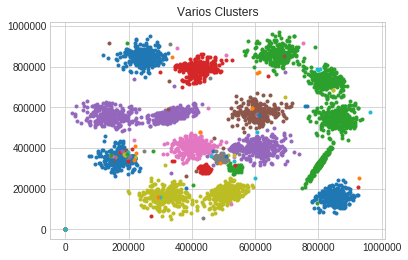
\includegraphics[scale=0.44]{experimentos/variosClusters}
	\end{minipage}\qquad
	\centering
	\begin{minipage}[t]{.3\textwidth}
		\centering
		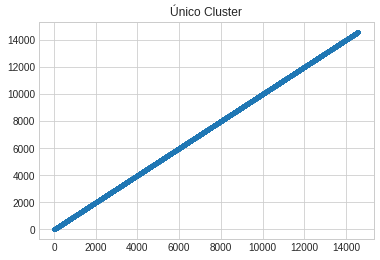
\includegraphics[scale=0.44]{experimentos/unicoCluster}
	\end{minipage}\qquad
\end{figure}	

\textbf{Nota}: Los puntos de la curva representan el promedio de ciclos de reloj de 10 ejecuciones por punto. Para cada grafo, desde 0 hasta 6500 se generaron datos en intervalos de 325 puntos, luego se genero información para 11500 puntos y por último para 14600 puntos.

\vspace{10 pt}

Los puntos a evaluar son:
\begin{itemize}
\item Performance entre Kruskal y Kruskal con path compression con varios clusters.
\item Performance entre Kruskal y Kruskal con path compression con un único cluster.
\item Evaluación de Kruskal con cota.
\end{itemize}


\subsubsubsection{Performance con varios clusters}


Al utilizar un grafo de 14600 puntos repartido en varios clusters como se pudo observar en la figura, se puede ver que cada cluster no contiene muchos puntos. Si bien, la alternativa de kruskal con path compression permite acceder al representante de un cluster en  $\mathcal{O}(1)$, al tratarse de clusters con pocos puntos, se espera que haya una diferencia mínima en los ciclos de reloj.

\begin{figure}[H]
	\centering
	\begin{minipage}[t]{.3\textwidth}
		\centering
		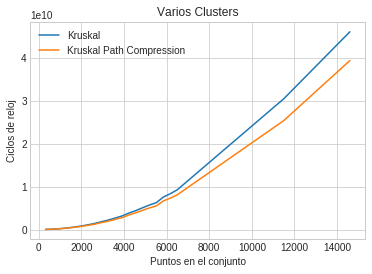
\includegraphics[scale=0.48]{experimentos/variosNormal}
	\end{minipage}
\end{figure}

Si bien la cantidad de ciclos de reloj entre una implementación y la otra comienzan a distanciarse a medida que se incrementan los puntos, la diferencia es mínima y se puede comprobar que la implementación con path compression se resuelve en menos ciclos.


\subsubsubsection{Performance con un único cluster}

Al utilizar el grafo de 14600 puntos repartido en un único cluster se espera que la optimización de path compression sea más visible y haya una mayor diferencia en la ejecución de cada algoritmo. 

\begin{figure}[H]
	\centering
	\begin{minipage}[t]{.3\textwidth}
		\centering
		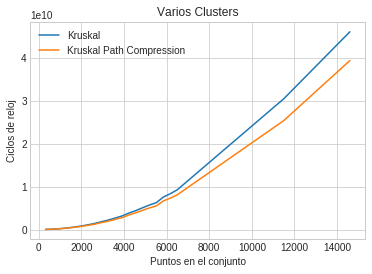
\includegraphics[scale=0.48]{experimentos/variosNormal}
	\end{minipage}
\end{figure}

Como se puede observar en la figura, los ciclos de reloj para cada algoritmo se distancian con una mayor diferencia que el caso anterior. Esto se debe a que la implementación normal de kruskal debe recorrer todo el arreglo de representantes, equivalente a recorrer todos los puntos ya analizados, para obtener el representante del cluster, que es único. En cambio, en el grafo anterior, los clusters contenían menos puntos, por ello la diferencia no era tan notable. En la última parte del grafo es posible ver como la pendiente de la ejecución para kruskal crece más rapidamente que para kruskal con path compression.


\subsubsubsection{Evaluación de cota}

La complejidad de ambas implementaciones es la misma, por eso se espera que ante la cota tomada, ambos pasen a estar por debajo de la misma a partir de un cierto valor.

\begin{figure}[H]
	\centering
	\begin{minipage}[t]{.3\textwidth}
		\centering
		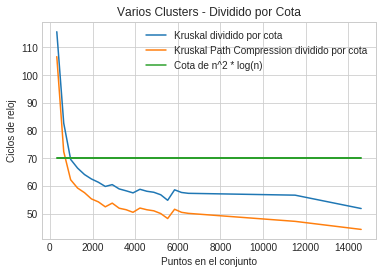
\includegraphics[scale=0.44]{experimentos/variosDivididoPorCota}
	\end{minipage}
	\centering
	\begin{minipage}[t]{.3\textwidth}
		\centering
		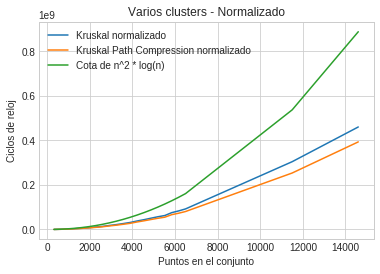
\includegraphics[scale=0.44]{experimentos/variosNormalizadoCota}
	\end{minipage}
\end{figure}

Como podemos ver, la funcion converge a un valor constante al dividirla por la complejidad planteada, lo cual demuestra que cumple con dicha cota.